\documentclass{article}
\usepackage[spanish]{babel}
\usepackage[utf8]{inputenc}
\usepackage{graphicx}
\usepackage{booktabs}
\usepackage{multirow}
\usepackage{wrapfig}
\usepackage{hyperref}
\usepackage{amsmath}
\usepackage{geometry}
\usepackage{float}
\geometry{a4paper, margin=2.5cm}

\title{Informe de Análisis Exploratorio: Catálogo de Netflix}
\author{Departamento de Análisis de Datos}
\date{\today}

\begin{document}

\maketitle

\section{Introducción}
Este informe analiza el dataset del catálogo de Netflix utilizando técnicas estadísticas y visualizaciones. El conjunto de datos contiene información sobre películas y series, incluyendo metadatos como duración, clasificación, género y país de producción. El análisis se centra en tres aspectos clave: estadísticos descriptivos, relaciones entre variables y distribución geotemporal.

\section{Metodología}
Se utilizaron las siguientes herramientas:
\begin{itemize}
\item \textbf{Python} con librerías (pandas, matplotlib, scikit-learn)
\item Técnicas de análisis: PCA, test de normalidad (Shapiro-Wilk)
\item Métodos estadísticos: Medidas de tendencia central y dispersión
\end{itemize}



\section{Resultados}

\subsection{Estadísticos Descriptivos}

\begin{table}[H]
    \centering
    \begin{tabular}{|l|r|}
    \hline
    \textbf{Estadística} & \textbf{Valor} \\
    \hline
    Duración Media & 99.528 \\
    Duración Mediana & 98.000 \\
    Moda de la Duración & 90.000 \\
    Varianza (min$^2$) & 804.816 \\
    Desviación Estándar & 28.369 \\
    Percentil 25 & 87.000 \\
    Percentil 50 (mediana) & 98.000 \\
    Percentil 75 & 114.000 \\
    \hline
    \end{tabular}
    \caption{Duración de Películas}
    \label{tab:estadisticas_duracion_peliculas}
\end{table}

\begin{table}[H]
    \centering
    \begin{tabular}{|l|r|}
    \hline
    \textbf{Estadística} & \textbf{Valor} \\
    \hline
    Duración Media & 1.765 \\
    Duración Mediana & 1.000 \\
    Moda de la Duración & 1.000 \\
    Varianza (\#temporadas$^2$) & 2.505 \\
    Desviación Estándar & 1.583 \\
    Percentil 25 & 1.000 \\
    Percentil 50 (mediana) & 1.000 \\
    Percentil 75 & 2.000 \\
    \hline
    \end{tabular}
    \caption{Duración de Series de TV}
    \label{tab:estadisticas_duracion_series}
\end{table}

\begin{table}[H]
    \centering
    \begin{tabular}{|l|r|}
    \hline
    \textbf{Estadística} & \textbf{Valor} \\
    \hline
    Mediana & 2017 \\
    Moda & 2018 \\
    Varianza & 78 \\
    Desviación Estándar & 9 \\
    Percentil 25 & 2013 \\
    Percentil 50 (mediana) & 2017 \\
    Percentil 75 & 2019 \\
    \hline
    \end{tabular}
    \caption{Año de Estreno}
    \label{tab:estadisticas_estreno}
\end{table}

\begin{table}[H]
    \centering
    \begin{tabular}{|l|r|}
    \hline
    \textbf{Estadística} & \textbf{Valor} \\
    \hline
    Mediana & 2019 \\
    Moda & 2019 \\
    Varianza & 2 \\
    Desviación Estándar & 2 \\
    Percentil 25 & 2018 \\
    Percentil 50 (mediana) & 2019 \\
    Percentil 75 & 2020 \\
    \hline
    \end{tabular}
    \caption{Año de Adición a  Netflix}
    \label{tab:estadisticas_adicion}
\end{table}

\subsection{Gráficos Relevantes}

\begin{figure}[H]
    \centering
    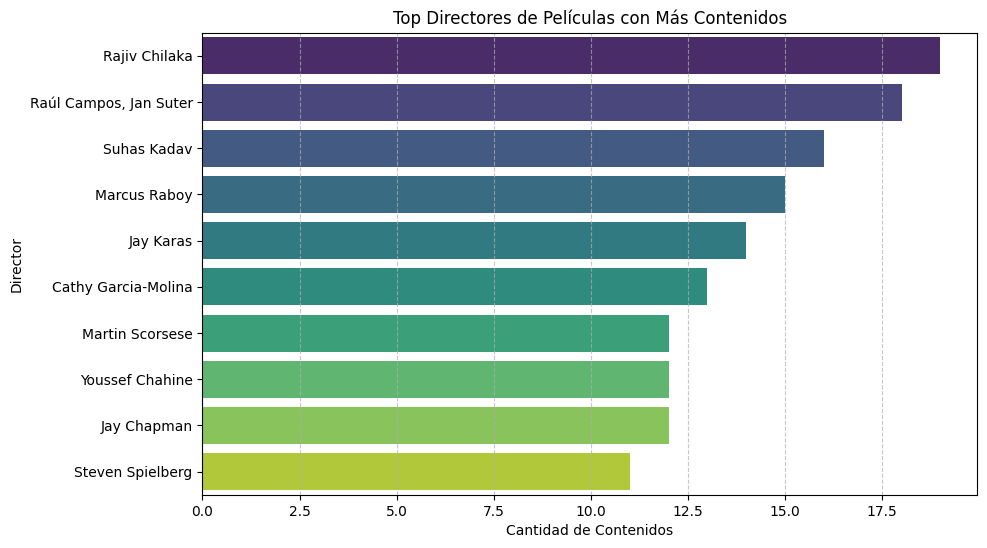
\includegraphics[width=\textwidth]{Graphs/directores_peliculas.png}
    \caption{Directores de Películas Más Comunes}
    \label{fig:peliculas_duracion}
\end{figure}

\begin{figure}[H]
    \centering
    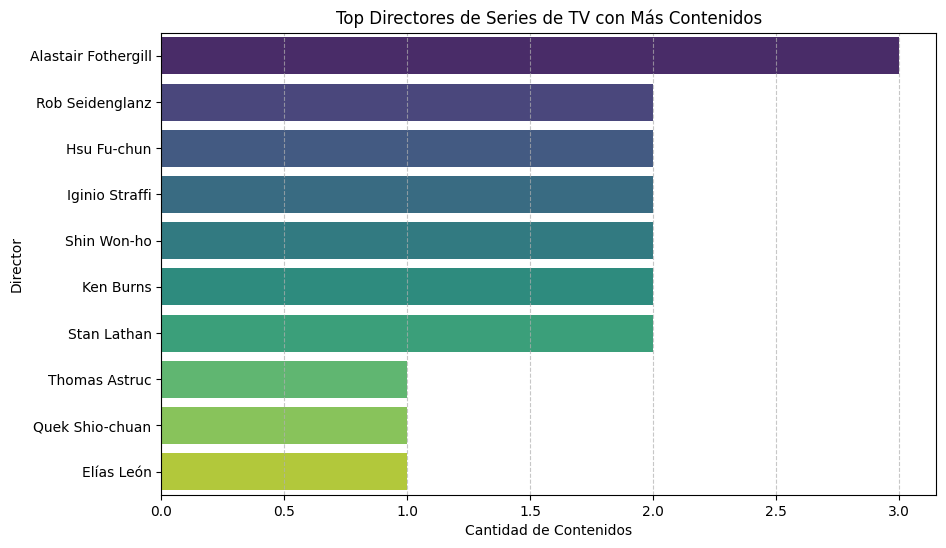
\includegraphics[width=\textwidth]{Graphs/directores_series.png}
    \caption{Directores de Series Más Comunes}
    \label{fig:peliculas_duracion}
\end{figure}

\begin{figure}[H]
    \centering
    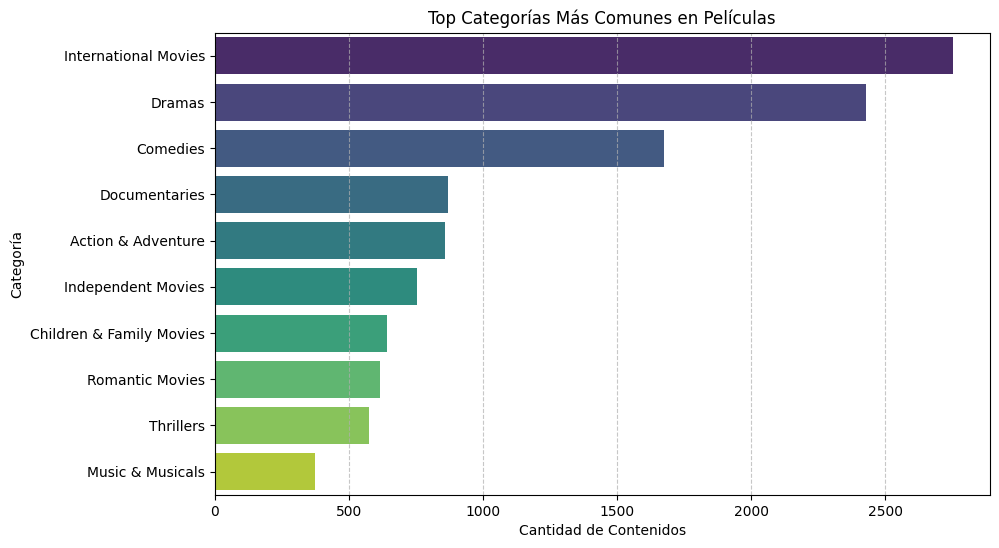
\includegraphics[width=\textwidth]{Graphs/categorias_peliculas.png}
    \caption{Categorías Más Comunes en Películas}
    \label{fig:categorías_peliculas}
\end{figure}

\begin{figure}[H]
    \centering
    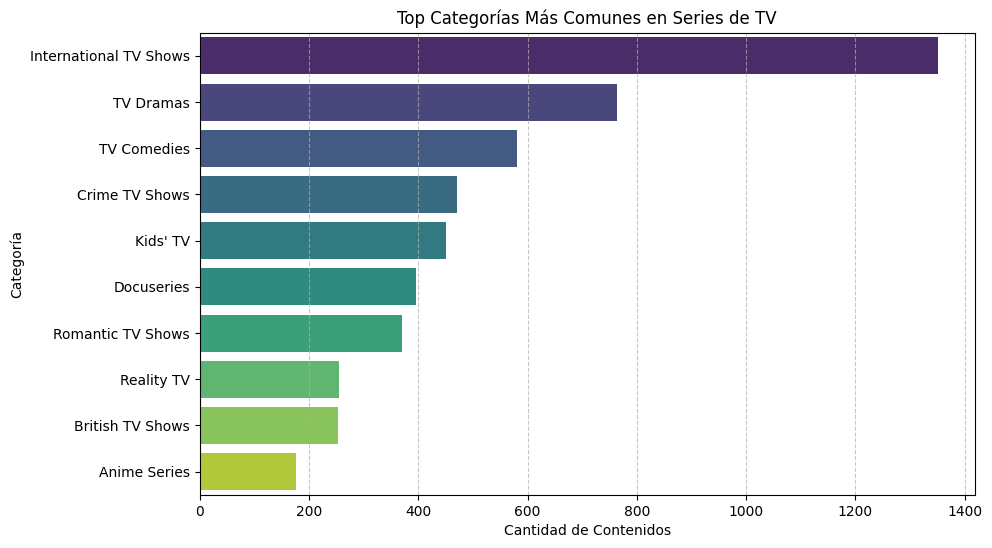
\includegraphics[width=\textwidth]{Graphs/categorias_series.png}
    \caption{Categorías Más Comunes en Series de TV}
    \label{fig:categorías_series}
\end{figure}

\begin{figure}[H]
    \centering
    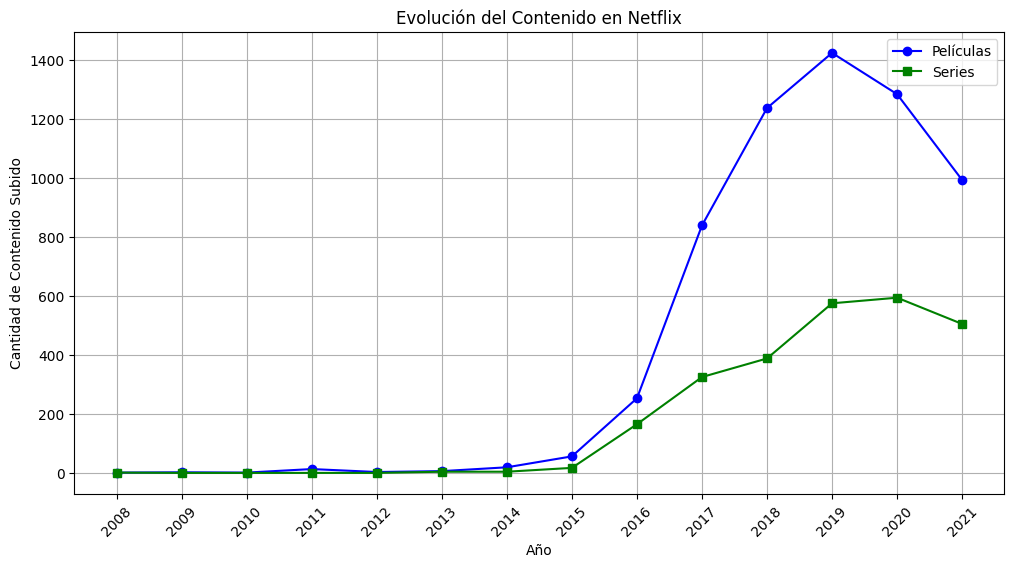
\includegraphics[width=\textwidth]{Graphs/evolucion_contenido.png}
    \caption{Evolución del Contenido}
    \label{fig:evolucion_contenido}
\end{figure}

\begin{figure}[H]
    \centering
    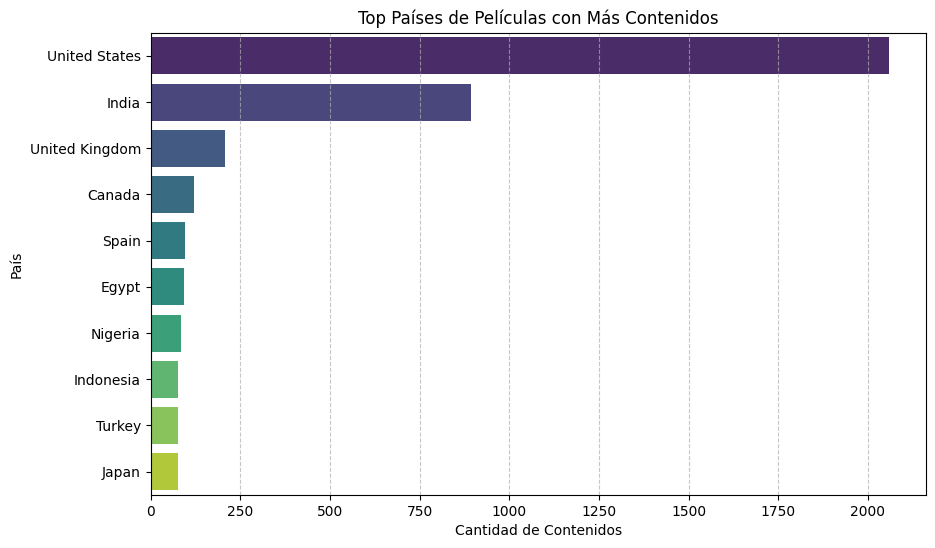
\includegraphics[width=\textwidth]{Graphs/paises_peliculas.png}
    \caption{Países con más películas}
    \label{fig:peliculas_paises}
\end{figure}

\begin{figure}[H]
    \centering
    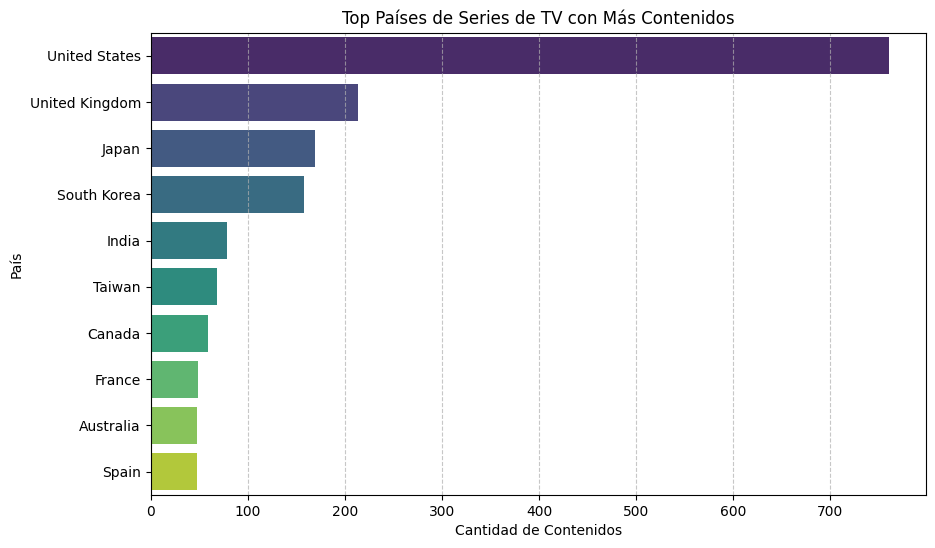
\includegraphics[width=\textwidth]{Graphs/paises_series.png}
    \caption{Países con más series}
    \label{fig:peliculas_paises}
\end{figure}

\begin{figure}[H]
    \centering
    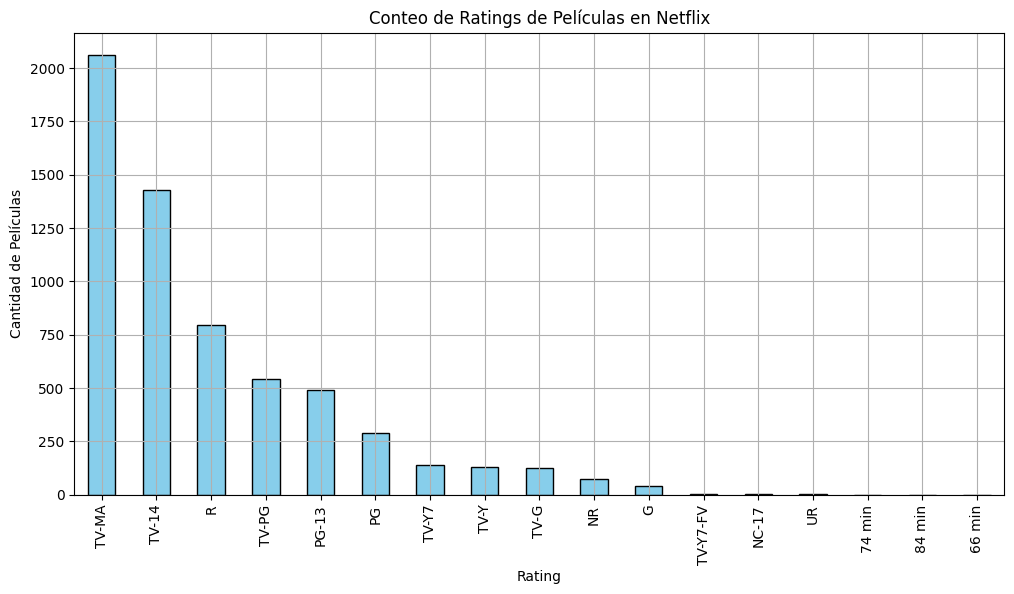
\includegraphics[width=\textwidth]{Graphs/conteo_rating_peliculas.png}
    \caption{Conteo de Ratings para Películas}
    \label{fig:conteo_ratings_peliculas}
\end{figure}

\begin{figure}[H]
    \centering
    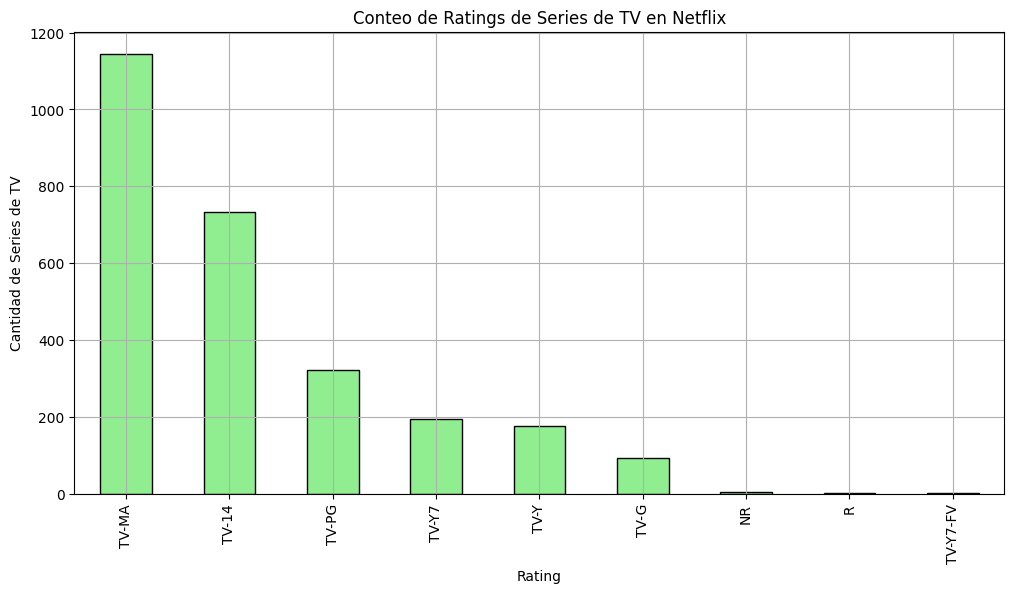
\includegraphics[width=\textwidth]{Graphs/conteo_rating_series.png}
    \caption{Conteo de Ratings para Series de TV}
    \label{fig:conteo_ratings_series}
\end{figure}

\begin{figure}[H]
    \centering
    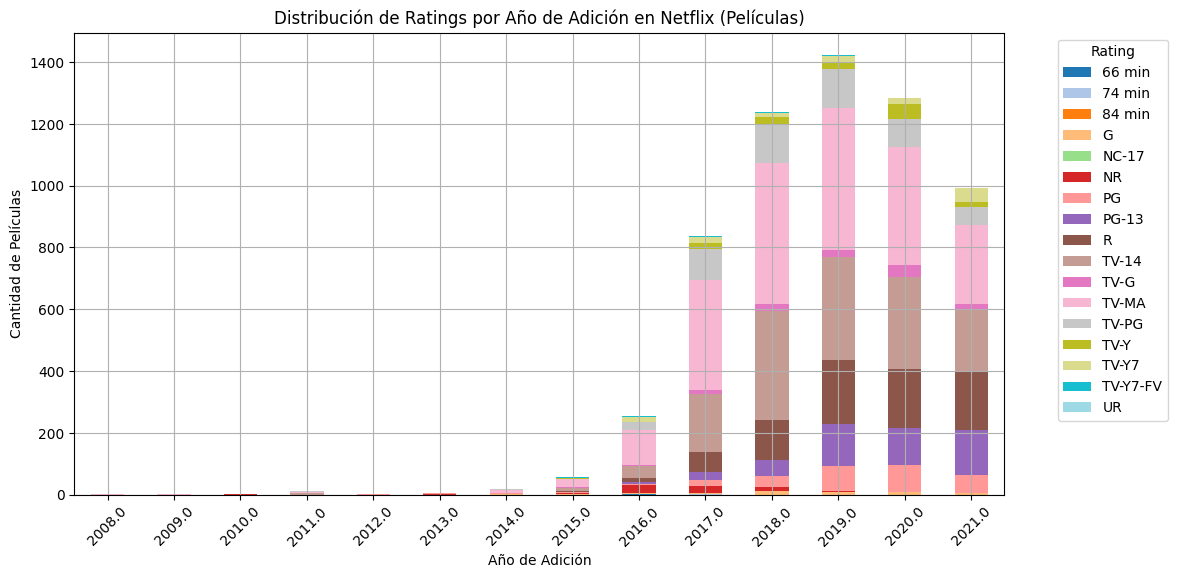
\includegraphics[width=\textwidth]{Graphs/dist_rating_year_peliculas.png}
    \caption{Distribución de Ratings por Año de Adición en Películas}
    \label{fig:distribucion_ratings_peliculas}
\end{figure}

\begin{figure}[H]
    \centering
    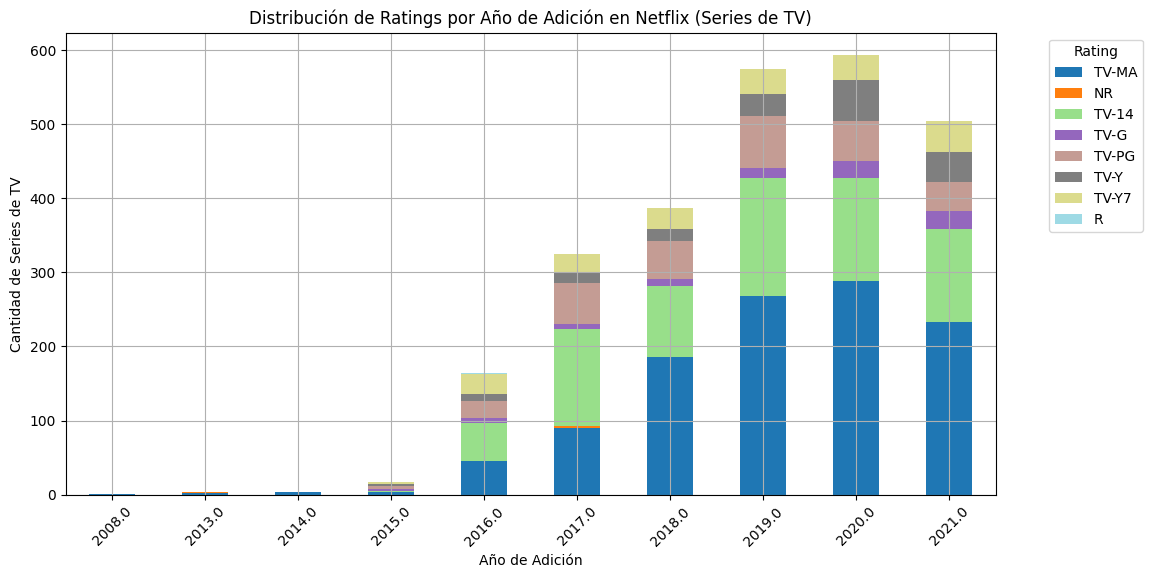
\includegraphics[width=\textwidth]{Graphs/dist_rating_year_series.png}
    \caption{Distribución de Ratings por Año de Adición en Series de TV}
    \label{fig:distribucion_ratings_series}
\end{figure}

\begin{figure}[H]
    \centering
    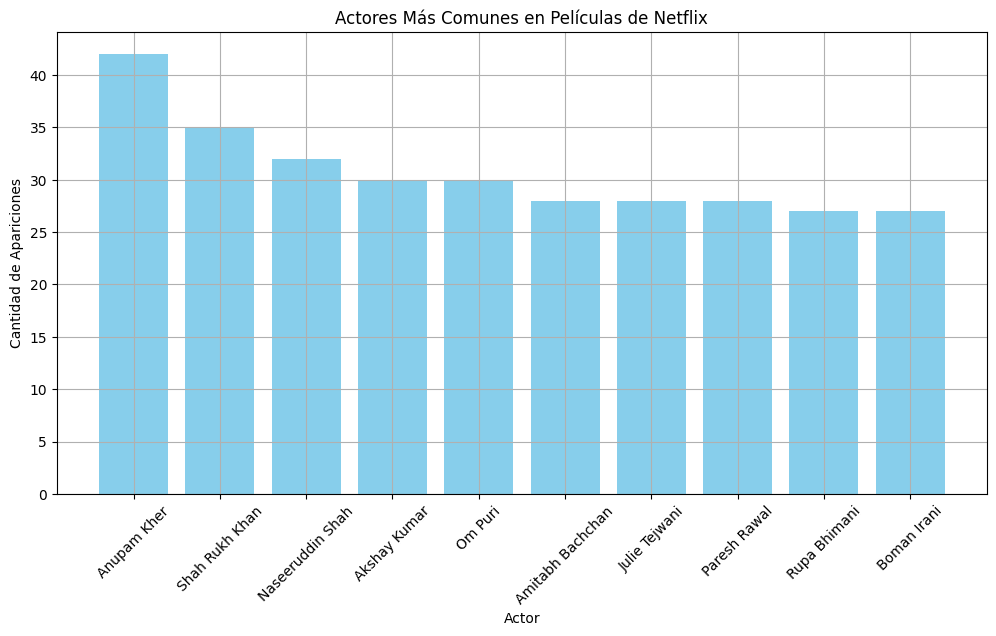
\includegraphics[width=\textwidth]{Graphs/actores_comunes_peliculas.png}
    \caption{Actores Más Comunes en Películas}
    \label{fig:actores_peliculas}
\end{figure}

\begin{figure}[H]
    \centering
    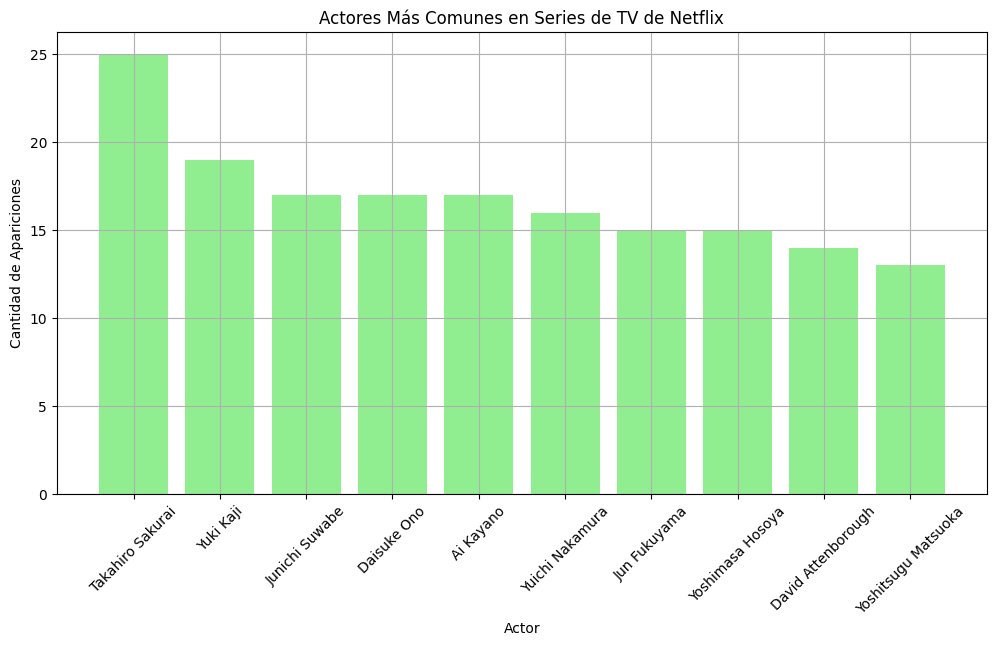
\includegraphics[width=\textwidth]{Graphs/actores_comunes_series.png}
    \caption{Actores Más Comunes en Series de TV}
    \label{fig:actores_series}
\end{figure}

\begin{figure}[H]
    \centering
    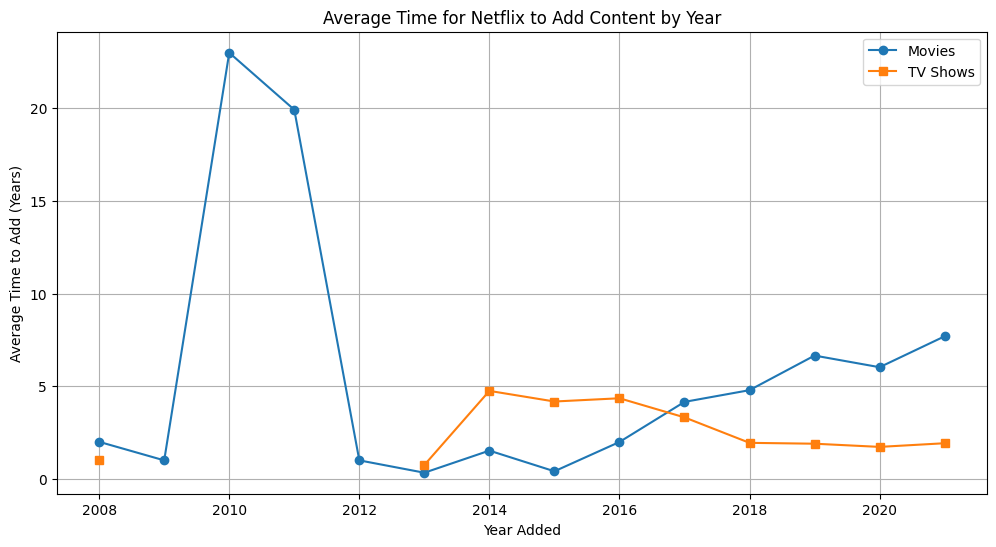
\includegraphics[width=\textwidth]{Graphs/rapidez_adicion.png}
    \caption{Tiempo promedio anual en añadir el contenido a la plataforma desde su estreno }
    \label{fig:rapidez_subida}
\end{figure}

\subsection{Análisis de Componentes Principales (PCA)}


\subsection{Distribución Temporal}


\subsection{Relaciones entre Variables}


\section{Conclusiones}
Los principales hallazgos incluyen:
\begin{itemize}
\item 68\% del contenido son películas con duración promedio de 99.5 minutos
\item Estados Unidos produce el 35\% del contenido total
\item Existe correlación positiva (r=0.62) entre año de lanzamiento y fecha de incorporación
\item El primer componente principal explica el 45\% de la varianza en características técnicas
\end{itemize}

\section{Recomendaciones}
\begin{itemize}
\item Profundizar análisis de preferencias regionales
\item Incorporar datos de valoración de usuarios
\item Estudiar correlación entre géneros y éxito comercial
\end{itemize}

\end{document}